% file: sims_0.tex
% created by Orbiter tikz interface
% creation date: Mon Nov 25 12:41:01 MST 2019
% DeviceCoordinates 0 0 300000 300000
% UserCoordinates 0 0 10000 10000
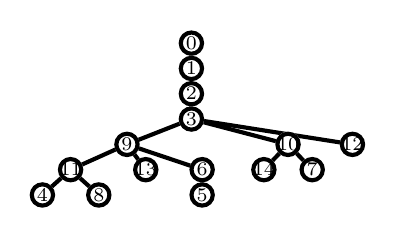
\begin{tikzpicture}[scale=0.45,line width = 1.5pt]
\draw [] (5,9.642) -- (5,8.928);
\draw [] (5,8.928) -- (5,8.214);
\draw [] (5,8.214) -- (5,7.5);
\draw [] (5,7.5) -- (3.181,6.785);
\draw [] (5,7.5) -- (7.727,6.785);
\draw [] (5,7.5) -- (9.545,6.785);
\draw [] (3.181,6.785) -- (1.59,6.071);
\draw [] (3.181,6.785) -- (3.71197,6.071);
\draw [] (3.181,6.785) -- (5.303,6.071);
\draw [] (7.727,6.785) -- (7.045,6.071);
\draw [] (7.727,6.785) -- (8.409,6.071);
\draw [] (1.59,6.071) -- (0.795,5.357);
\draw [] (1.59,6.071) -- (2.386,5.357);
\draw [] (5.303,6.071) -- (5.303,5.357);
\filldraw[color=white] (5,9.642) circle [radius = 0.3cm];
\draw (5,9.642) circle [radius = 0.3cm];
\draw (5,9.642) node{{\scriptsize 0}};
\filldraw[color=white] (5,8.928) circle [radius = 0.3cm];
\draw (5,8.928) circle [radius = 0.3cm];
\draw (5,8.928) node{{\scriptsize 1}};
\filldraw[color=white] (5,8.214) circle [radius = 0.3cm];
\draw (5,8.214) circle [radius = 0.3cm];
\draw (5,8.214) node{{\scriptsize 2}};
\filldraw[color=white] (5,7.5) circle [radius = 0.3cm];
\draw (5,7.5) circle [radius = 0.3cm];
\draw (5,7.5) node{{\scriptsize 3}};
\filldraw[color=white] (3.181,6.785) circle [radius = 0.3cm];
\draw (3.181,6.785) circle [radius = 0.3cm];
\draw (3.181,6.785) node{{\scriptsize 9}};
\filldraw[color=white] (7.727,6.785) circle [radius = 0.3cm];
\draw (7.727,6.785) circle [radius = 0.3cm];
\draw (7.727,6.785) node{{\scriptsize 10}};
\filldraw[color=white] (9.545,6.785) circle [radius = 0.3cm];
\draw (9.545,6.785) circle [radius = 0.3cm];
\draw (9.545,6.785) node{{\scriptsize 12}};
\filldraw[color=white] (1.59,6.071) circle [radius = 0.3cm];
\draw (1.59,6.071) circle [radius = 0.3cm];
\draw (1.59,6.071) node{{\scriptsize 11}};
\filldraw[color=white] (3.71197,6.071) circle [radius = 0.3cm];
\draw (3.71197,6.071) circle [radius = 0.3cm];
\draw (3.71197,6.071) node{{\scriptsize 13}};
\filldraw[color=white] (5.303,6.071) circle [radius = 0.3cm];
\draw (5.303,6.071) circle [radius = 0.3cm];
\draw (5.303,6.071) node{{\scriptsize 6}};
\filldraw[color=white] (7.045,6.071) circle [radius = 0.3cm];
\draw (7.045,6.071) circle [radius = 0.3cm];
\draw (7.045,6.071) node{{\scriptsize 14}};
\filldraw[color=white] (8.409,6.071) circle [radius = 0.3cm];
\draw (8.409,6.071) circle [radius = 0.3cm];
\draw (8.409,6.071) node{{\scriptsize 7}};
\filldraw[color=white] (0.795,5.357) circle [radius = 0.3cm];
\draw (0.795,5.357) circle [radius = 0.3cm];
\draw (0.795,5.357) node{{\scriptsize 4}};
\filldraw[color=white] (2.386,5.357) circle [radius = 0.3cm];
\draw (2.386,5.357) circle [radius = 0.3cm];
\draw (2.386,5.357) node{{\scriptsize 8}};
\filldraw[color=white] (5.303,5.357) circle [radius = 0.3cm];
\draw (5.303,5.357) circle [radius = 0.3cm];
\draw (5.303,5.357) node{{\scriptsize 5}};
\end{tikzpicture}
